\part{Misura della costante di Rydberg}
\section{Scopo e strumentazione}
	L'obiettivo di questa seconda parte è di misurare la costante di Rydberg, per farlo verranno misurate le righe di emissione di una lampada all'idrogeno per mezzo di uno spettroscopio a reticolo. Preliminarmente lo strumento dovrà essere calibrato attraverso la misura della viga verde di una lampada al mercurio di lunghezza d'onda nota.
	Infine, con lo scopo di testare precisione e risoluzione dello strumento, si procederà alla misura della lunghezza d'onda del doppietto giallo di una lampada al sodio.

La strumentazione utilizzata si compone di:
\begin{itemize}
	\item uno spettroscopio a reticolo il cui goniometro ha in teoria una risoluzione di $30"$;
	\item una lampada al mercurio del quale si assume di conoscere la lunghezza d'onda delle righe spettrali e che servità per la calibrazione dell'apparato;
	\item una lampada all'idrogeno e una al sodio.
\end{itemize}

Si riporta in \figurename{ \ref{fig:reticolo}} uno schema dell'apparato.
sperimentale impiegato. 
\begin{figure} [H]
	\centering
	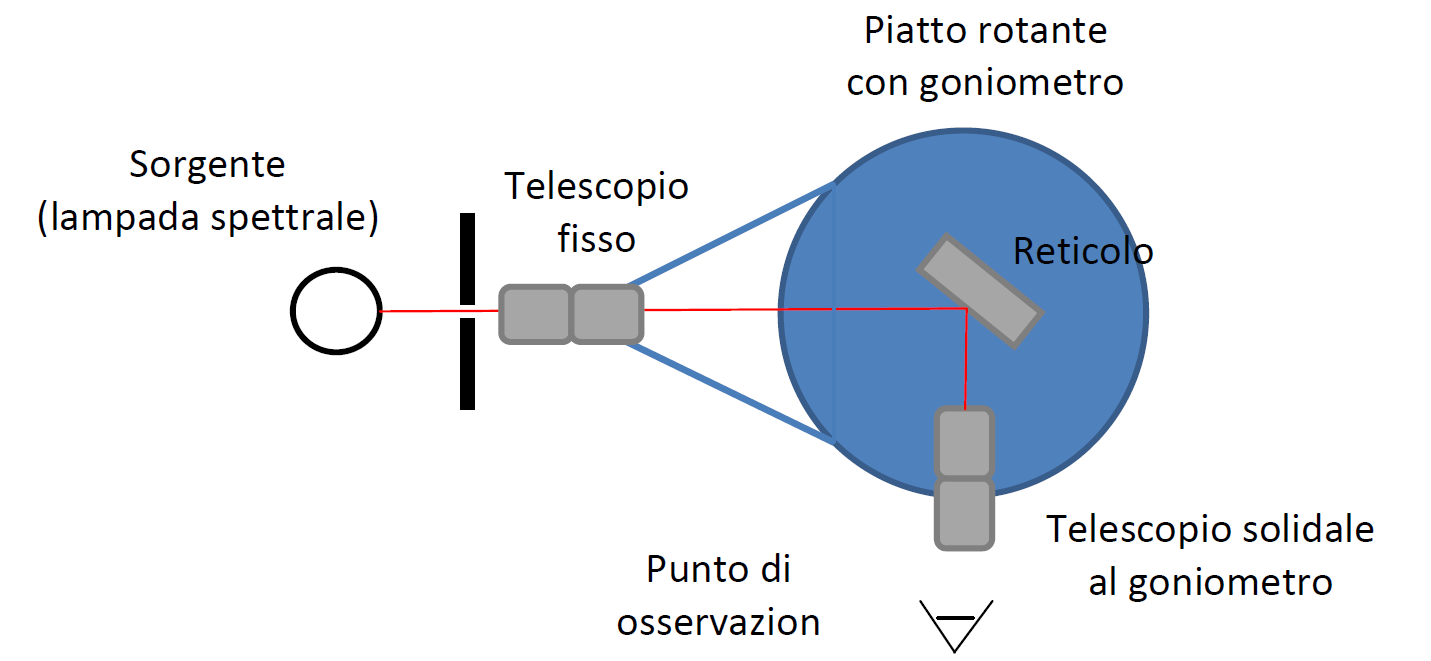
\includegraphics[width=0.6\textwidth]{../Figs-tabs/reticolo.png}
	\caption{Schema dell'apparato impiegato nella seconda parte dell'esperienza.}
	\label{fig:reticolo}
\end{figure}
